\documentclass[aspectratio=169,hyperref={implicit=true}]{beamer}
%\documentclass{beamer}
%%%CHOOSE ASPECT RATIO ABOVE%%%

\usetheme[showallsubsections]{UH-Slides-SEG2022}
\addbibresource{bib/ref_nn.bib}
\addbibresource{bib/ref_superrs.bib}

% \usepackage[utf8]{inputenc} % Not necessary.
% \usepackage[american]{babel} % Have been embedded in the theme.

%\setbeameroption{show notes} % Use this command to produce notes for slides.

\title[Demo]{Beamer Example}

\setTitleColor{white} % Choose between UHRed, UHBlue, UHPink, UHGreen, UHLBlue, UHIvory, SEGNavy, SEGBlue, SEGRed, SEGYellow, IMAGEPrimary, IMAGESecondary, IMAGETertiary, IMAGEQuaternary
\setTitleImage{title-2022.jpg}
%\setTitleImage[width=\paperwidth]{title-2021.jpg} % or title-2021-2.jpg
\setFinalColor{white} % Choose between UHRed, UHBlue, UHPink, UHLBlue, UHIvory, SEGNavy, SEGBlue, SEGRed, SEGYellow, IMAGEPrimary, IMAGESecondary, IMAGETertiary, IMAGEQuaternary
\setFinalImage{cullen.jpg}
%\setTitleLogo[1.8in]{seg-2022-alt.png} % If not set, we would use seg-202x-alt.png
%\setFirstLogo{seg-2022.png} % If not set, we would use seg-202x.png
%\setSecondLogo{seg-2021.png} % If not set, the second logo would be left blank.
\author{Yuchen Jin}
\subtitle{A beamer template for SEG-2021/UH}
\date{\today} % Could be replaced by a manually specified date: \DTMdate{YYYY-MM-DD}
%\date{\DTMdate{2022-09-02}}
\institute[Department of ECE]{University of Houston\\Department of ECE}

\AtBeginSection[]
{
  \begin{frame}<beamer> % with <beamer> => doesn't appear in handout mode
    \frametitle{Outline} %% Put the title you want, or none!
    %\tableofcontents[currentsection,currentsubsection]
      %\setcounter{unbalance}{\value{unbalanceSet}}
      \tableofcontents[currentsection]
      %\vspace{12em}
      %\mbox{}
  \end{frame}
}

\begin{document}

\titleframe

\begin{frame}

\frametitle{Outline}
\tableofcontents[currentsection]

\end{frame}

\section{Introduction}

\begin{frame}
  
\frametitle{Introduction}

\begin{itemize}
  \item This is the template for UH slides, which includes:
  \begin{itemize}
    \item \textbf{Table}: Check \cref{tab:params}.
    \item \textbf{Figure}: Check \cref{fig:ex1:resD}.
    \item \textbf{Block and Equation}: Check \eqref{fml:eq1:partialW}.
    \item \textbf{Theorem}: Check \cref{thm:th1}.
    \item \textbf{Algorithm}: Check \cref{alg::Algorithm}.
    \item \textbf{Slide transition}: Check \cref{sec:slidetrans}.
  \end{itemize}
  \item And here we would like to test the references: \textit{Zeiler et al.}\footcite{Zeiler5539957}, \textit{Yang et al.}~\footcite{Yang6175956}, \textit{Dong et al.}~\footcite{Dong7115171}.
\end{itemize}

\end{frame}

\section{Test}

\subsection{Table test}
\begin{frame}
\frametitle{Test}
\framesubtitle{Table test}

\begin{itemize}
  \item Test table, which is shown in \cref{tab:params}.
\end{itemize}

\begin{table}[htbp]
  \centering
  \normalsize
  \caption[Parameters of Daubechies's filter.]{Parameters of \textit{Daubechies}'s filter.}
  \label{tab:params}
  \begin{tabular}{|c|c|c|}
    \hline
    $n$ & $h[n]$ & $g[n]$ \\ \hline
    0 &  0.3327 & -0.0352 \\ \hline
    1 &  0.8069 & -0.0854 \\ \hline
    2 &  0.4599 &  0.1350 \\ \hline
    3 & -0.1350 &  0.4599 \\ \hline
    4 & -0.0854 & -0.8069 \\ \hline
    5 &  0.0352 &  0.3327 \\ \hline
  \end{tabular}
\end{table}

\end{frame}

\subsection{Figure test}

\begin{frame}

\frametitle{Test}
\framesubtitle{Figure test}

\begin{itemize}
  \item Test inner subgraphs, i.e. \cref{fig:ex1:resD:a} and \cref{fig:ex1:resD:b}.
\end{itemize}

\begin{figure}[htbp]
  \centering
  \subfigure[$D=1$]{ \label{fig:ex1:resD:a}
    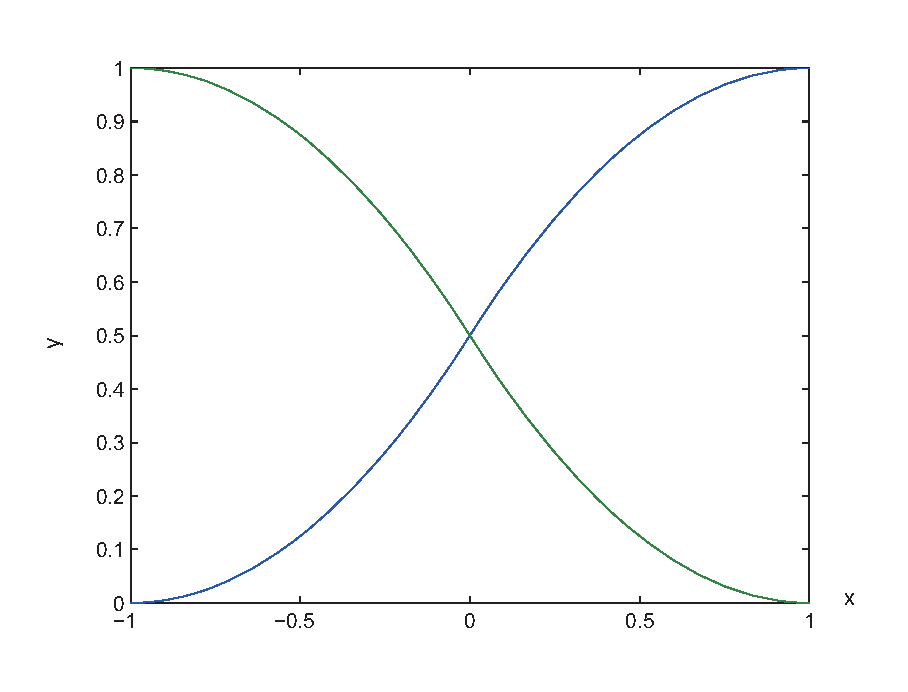
\includegraphics[width = 0.3\textwidth]{test1}
    \DeclareGraphicsExtensions.
  }
  \subfigure[$D=0.5$]{ \label{fig:ex1:resD:b}
    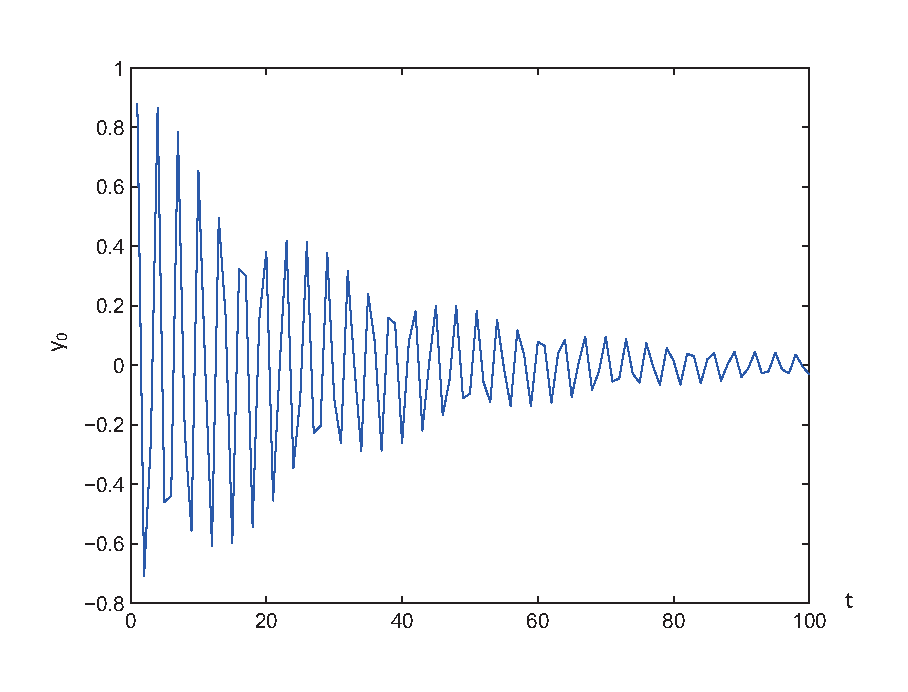
\includegraphics[width = 0.3\textwidth]{test2}
    \DeclareGraphicsExtensions.
  }
  \DeclareGraphicsExtensions.
  \caption{Test graphs.}\label{fig:ex1:resD}
\end{figure}

\end{frame}

\subsection{Equation test}

\begin{frame}

\frametitle{Test}
\framesubtitle{Equation test}

\begin{itemize}
  \item Test blocked equations, i.e. \eqref{fml:eq1:partialW}, \eqref{fml:eq1:partialb}.
\end{itemize}

\begin{block}{SVM loss function} \label{blc:eq1}
  Here we show a simple example of subequations in \eqref{fml:eq1:partialW}:
  \begin{subequations}
    \renewcommand{\theequation}
    {\theparentequation-\arabic{equation}}
    \begin{align}
    \frac{\partial \mathcal{L}(\mathbf{w},~b)}{\partial \mathbf{w}} &= \mathbf{w} + C \sum\limits_i\frac{\partial \ell_i}{\partial \mathbf{w}}, \label{fml:eq1:partialW}\\
    \frac{\partial \mathcal{L}(\mathbf{w},~b)}{\partial b} &= C \sum\limits_i\frac{\partial \ell_i}{\partial b}, \label{fml:eq1:partialb}
    \end{align}
  \end{subequations}
\end{block}

\end{frame}

\subsection{Theorem test}

\begin{frame}

\frametitle{Test}
\framesubtitle{Theorem test}

\begin{itemize}
  \item Test theorems, i.e. \cref{thm:th1} and \cref{thm:th2}.
\end{itemize}

\begin{columns}
  \begin{column}{.44\textwidth}
    \begin{theorem}[Example Theorem 1] \label{thm:th1}
      Nam dui ligula, fringilla a, euismod
      sodales, sollicitudin vel, wisi. Morbi
      auctor lorem non justo. Nam lacus
      libero, pretium at, lobortis vitae,
      ultricies et, tellus.
    \end{theorem}
  \end{column}
  \begin{column}{.52\textwidth}
    \begin{theorem}[Example Theorem 2] \label{thm:th2}
      Quisque ullamcorper placerat ipsum.
      Cras nibh. Morbi vel justo vitae lacus
      tincidunt ultrices. Lorem ipsum dolor
      sit amet, consectetuer adipiscing elit.
      In hac habitasse platea dictumst.
      Integer tempus convallis augue.
    \end{theorem}
  \end{column}
\end{columns}

\end{frame}

\subsection{Algorithm test}

\begin{frame}

\frametitle{Test}
\framesubtitle{Algorithm test}

\begin{itemize}
  \item Test algorithm, i.e. \cref{alg::Algorithm}.
\end{itemize}

\begin{algorithm}[H]
  \caption{DWT Algorithm}
  \label{alg::Algorithm}
  \begin{algorithmic}[1]
    \REQUIRE Sequence $\mathbf{x}$ in time domain
    \ENSURE Sequence $\hat{\mathbf{x}}$ in wavelet domain
    % if-then-else
    \STATE N = $\left\lfloor \log_2 (\mathrm{length}(\mathbf{x})) \right\rfloor$;
    \STATE $\mathbf{c}_{N} = \mathbf{x},~ \hat{\mathbf{x}} = \varnothing$;
    \FOR{$i$ from $1$ to $N$}
    \STATE $\mathbf{c}_{N-i},~\mathbf{d}_{N-i}~=~\mathrm{analysis\_filter}(\mathbf{c}_{N-i+1})$;
    \STATE insert $\mathbf{d}_{N-i}$ at the beginning of $\hat{\mathbf{x}}$.
    \ENDFOR
  \end{algorithmic}
\end{algorithm}
\end{frame}

\subsection{Slide transition test}

\begin{frame}

\frametitle{Test}
\framesubtitle{Slide transition test}
\label{sec:slidetrans}

\begin{columns}
  \begin{column}{.48\textwidth}
    \begin{itemize}
      \item<1-> This is transition test, let's begin:
      \begin{itemize}
        \item<2-> This is the first item.
        \item<3-> This is the second item.
        \item<4-> This is the third item.
      \end{itemize}
      \item<5-> We will show 3 items simultaneously.
      \begin{itemize}
        \item<6-> This is the first item.
        \item<6-> This is the second item.
        \item<6-> This is the third item.
      \end{itemize}
    \end{itemize}
  \end{column}
  \begin{column}{.48\textwidth}
    \only<7->{
    \begin{figure}[htbp]
      \centering
      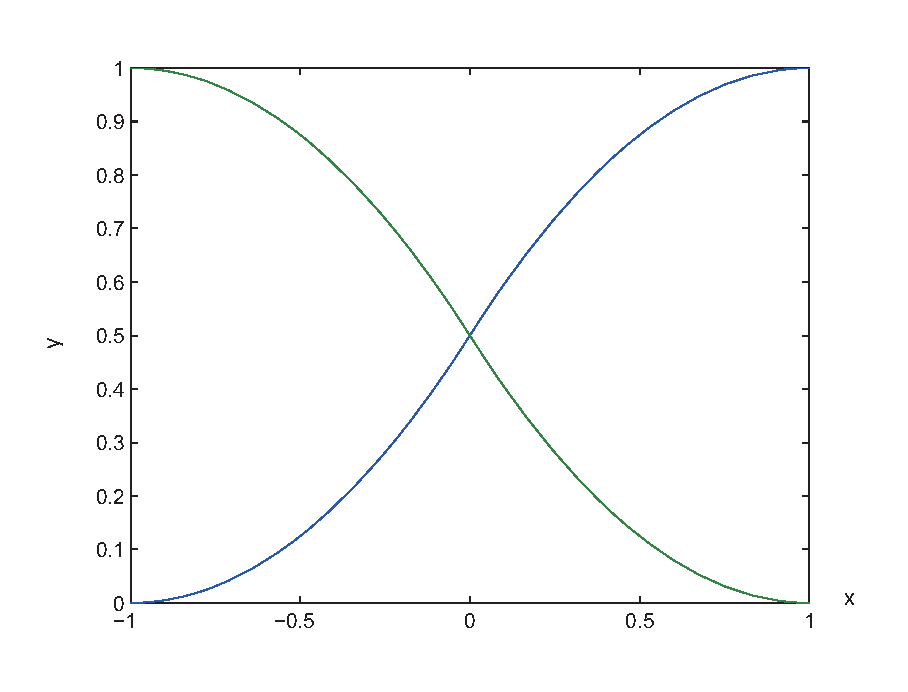
\includegraphics[width = 0.7\columnwidth]{test1}
      \DeclareGraphicsExtensions.
      \caption{Test graph.}\label{fig:ex2fig}
    \end{figure}
    }
  \end{column}
\end{columns}

\end{frame}

\finalframe[It's time for Q\&A.]

\end{document}
